\documentclass[12pt]{article}
\usepackage{graphicx, epstopdf}

\begin{document}
\title{Summary report of rejection email analysis}
\author{Davide Chiuchiu}

\maketitle

\section{Scope}
This document contains my findings on the corpus of emails that I received during my job search. The email database contains 
\begin{itemize}
	\item emails that confirmed the application submission and possible next steps
	\item emails where companies rejected my candidacy
	\item emails with feedback on how I could become a better candidate.
\end{itemize}

\section{I received more confirmation emails than rejection emails}
Overall, I received more emails which confirmed the reception of my candidacy than emails where my candidacy was rejected (see Figure \ref{fig:email_type_distribution}). This highlight that I have active review process at the moment, but also that some companies practice ghosting. Note also that only a few of the received emails corresponds to feedback. This means that I will ignore feedback emails when I will attempt machine learning on this dataset.

\begin{figure}[tb!]
	\center
	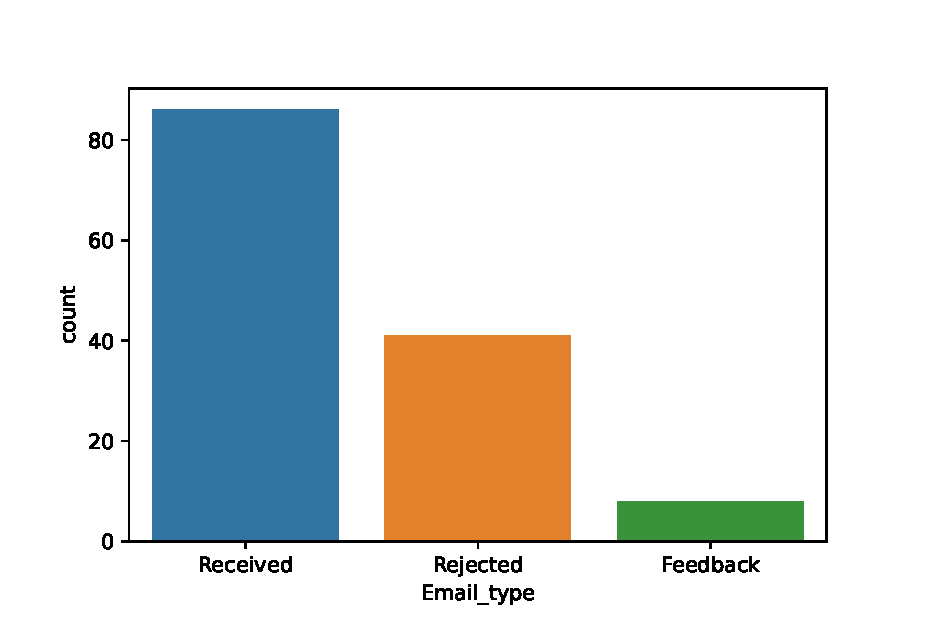
\includegraphics[width = 0.5\linewidth]{email_type_distribution.eps}
	\caption{I received more emails which confirms that my candidacy than  emails where my candidacy was rejected. Unfortunately, only a small subset of emails correspond to feedback from potential employers. \label{fig:email_type_distribution}}
\end{figure}

\section{Feedback might suffer because rejection emails tend to be quite short}
Unfortunately, rejection emails tend to be quite short and uninformative. Indeed, the emails which rejected one of my candidacy have the same number of sentences of the template emails which acknowledged my candidacy submission (\ref{fig:email_lengths}). This suggests that rejection emails are templates too, and those left me with no real understanding why I was rejected.

\begin{figure}
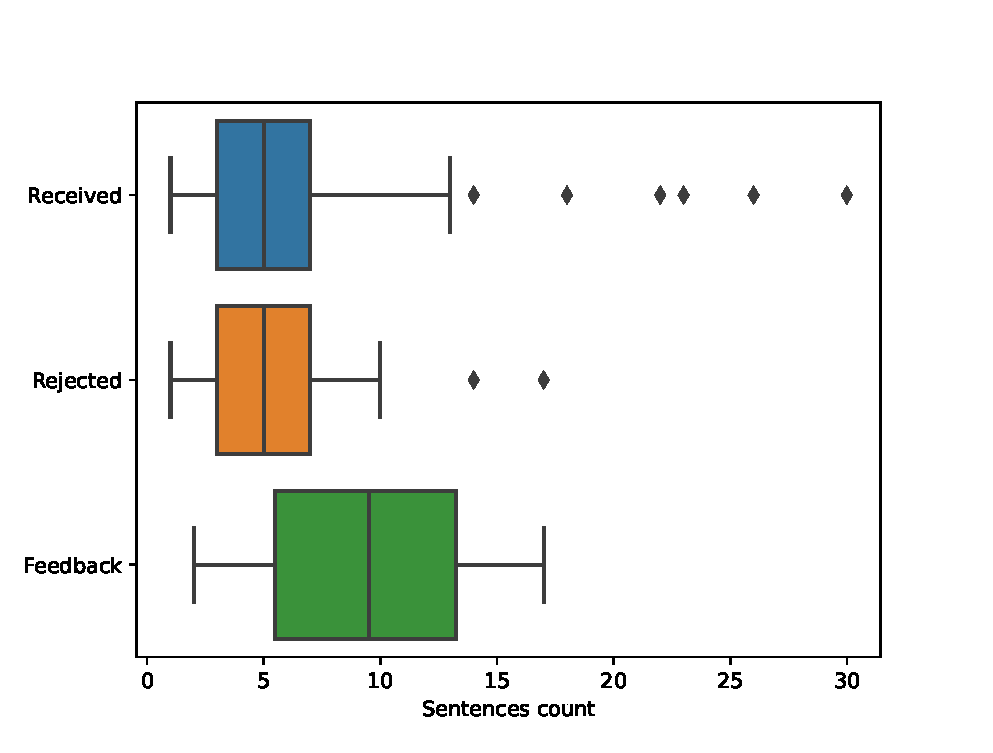
\includegraphics[width = \linewidth]{message_length_distribution.eps}
\caption{Emails where a candidacy was rejected corresponds to short templates with no real explanation why the candidacy was rejected in the end . \label{fig:email_lengths}}
\end{figure}

\section{Different email types can be recognized from different keywords}
A quick word count for each email type shows that keywords allows to distinguish emails where my application was rejected  from emails that confirmed the reception of my candidacy (see Figure \ref{fig:email_keywords}). More specifically, words like \emph{candidate} and \emph{unfortunately} uniquely identify emails where a candidacy was rejected. This makes classification with supervised learning possible even if the two email categories share some common keywords such as \emph{apply}, \emph{review} and \emph{team}.

\begin{figure}
    \center
	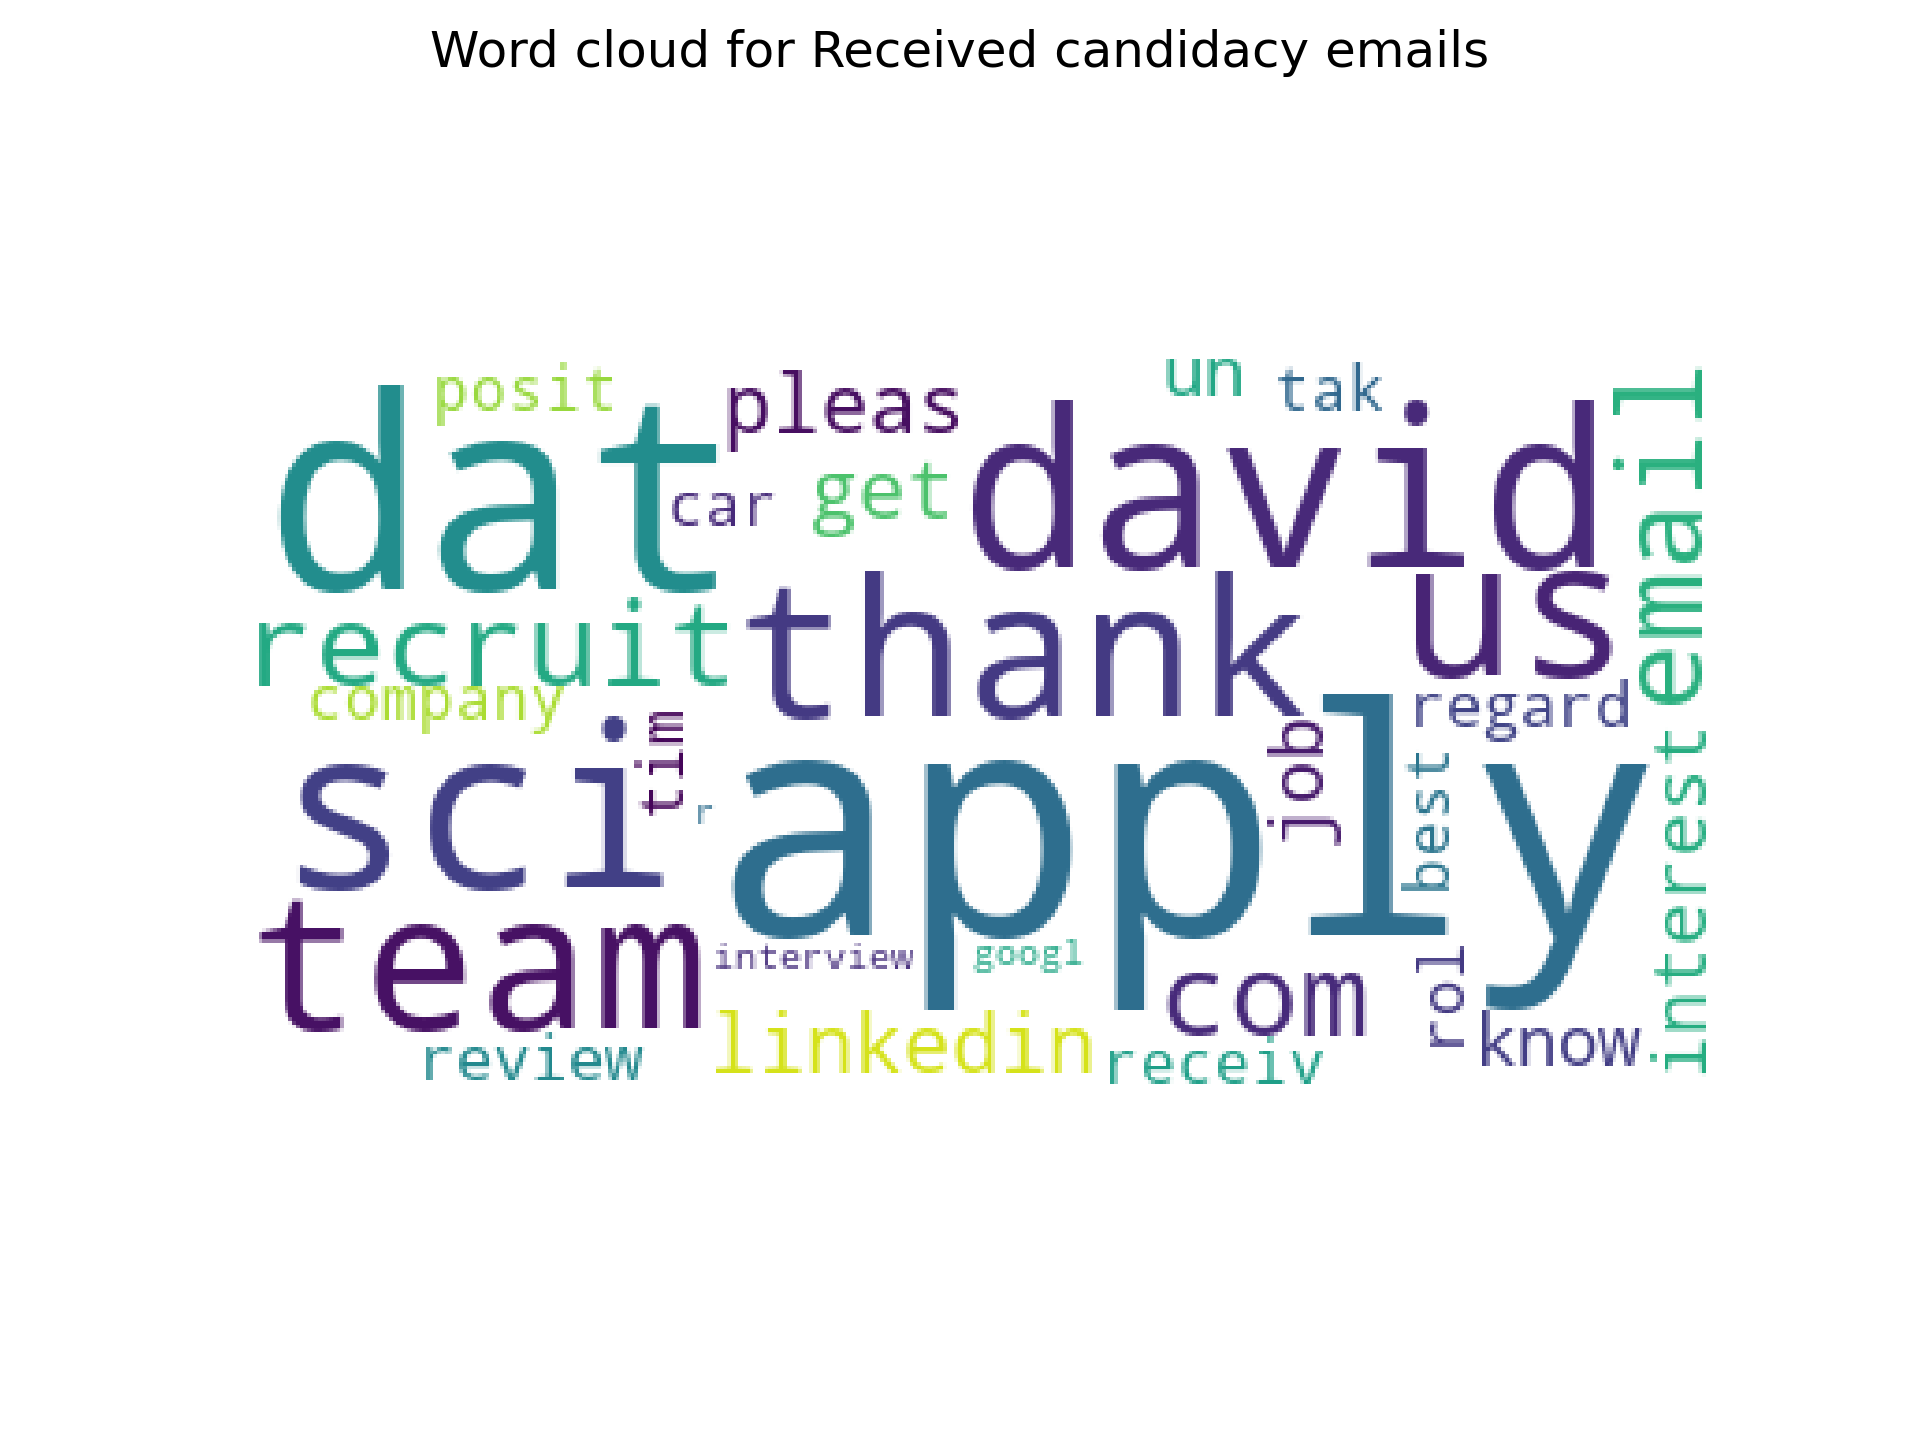
\includegraphics[width = \linewidth]{wordcloud_Received.png}
	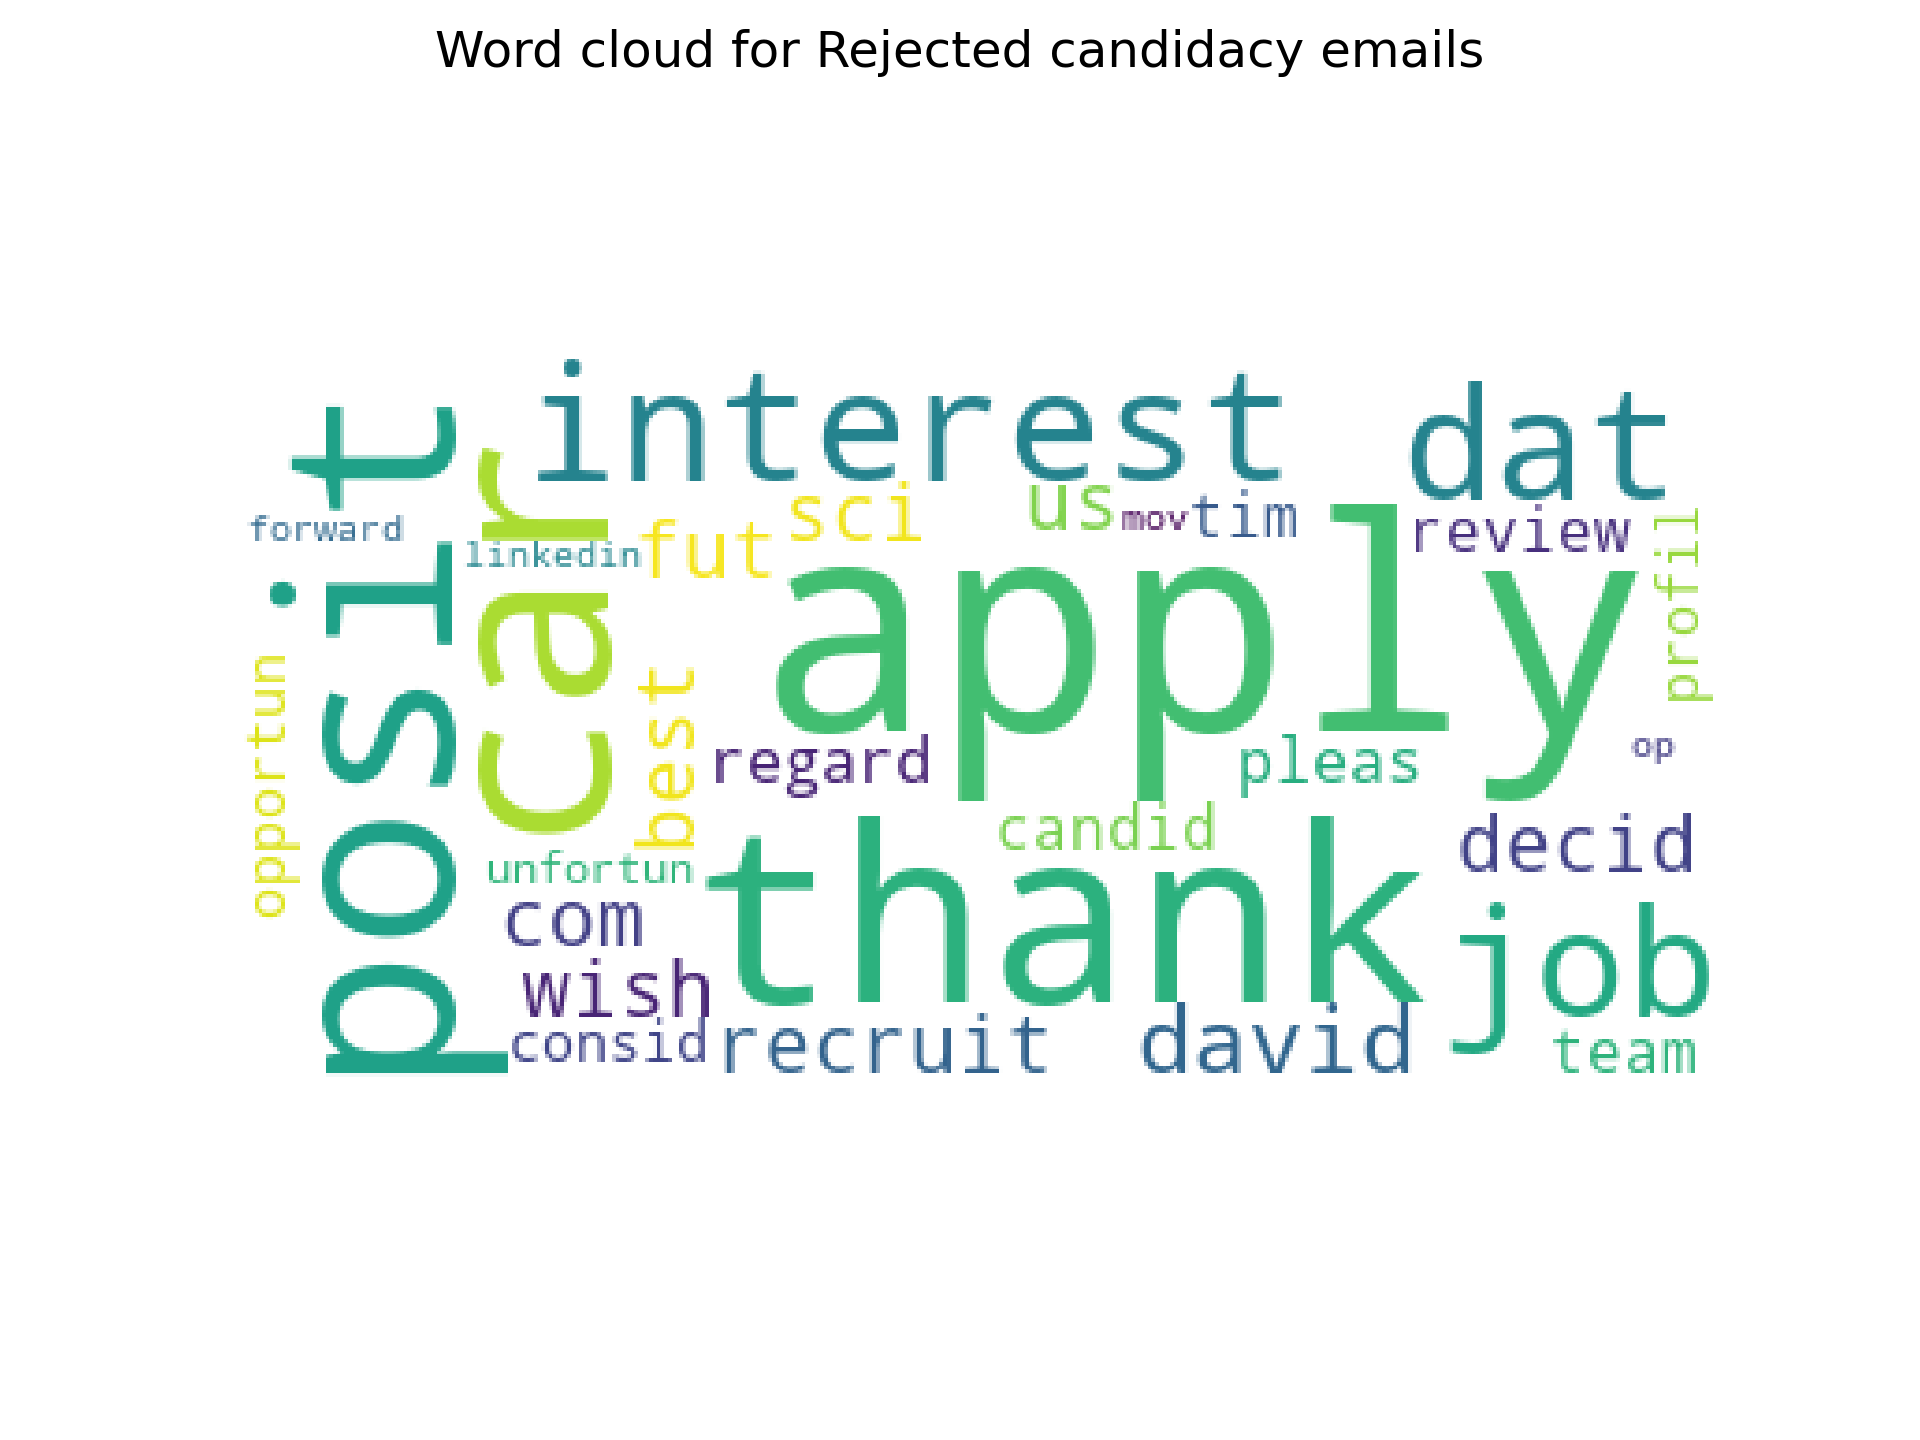
\includegraphics[width = \linewidth]{wordcloud_Rejected.png}
	\caption{Different email types can be identified by specific keywords.  \label{fig:email_keywords}}
\end{figure}

\end{document}